\chapter{Theoretical Framework}

Typical galaxies all around the Universe hold different structures such as stellar systems of between $ 10^{2} $ and $ 10^{6} $ stars which orbit their galactic core . We call these interesting systems star clusters and they are basically divided into three main types: Open Clusters, stellar associations and \textbf{Globular Clusters}. Open clusters are stellar systems that can contain from hundreds to thousands of stars, they are formed continuously in the Galactic disk and most of them are relatively young (younger than 1 Gyr). Old open clusters are rare since their gravitational stability is very low and can be easily disrupted by gravitational shocks from passing interstellar gas clouds. It seems likely that most of the stars in the galactic disk were formed in open clusters that have dissolved since then. 

Stellar associations such as young associations of stars that can contain 10–100 massive stars of spectral class O and B, and are known as OB associations. These associations also contain hundreds or thousands of low- and intermediate-mass stars.

Globular clusters, the other important class of stellar systems, are much more interesting and we focus deeply on their properties and characteristics.  

\section{Globular Clusters}
 
Globular clusters are very massive stellar systems that can contain from thousands to millions of stars in a nearly spherical distribution spread over a volume of several tens to about 200 light years in diameter. These stellar systems are composed of old stars and they do not contain gas or dust. As an example the next figure shows M15 Globular Cluster, that was discovered by Jean-Dominique Maraldi in 1746 while he was studying the De Chéseaux comet.

\begin{figure}[H]
\centering
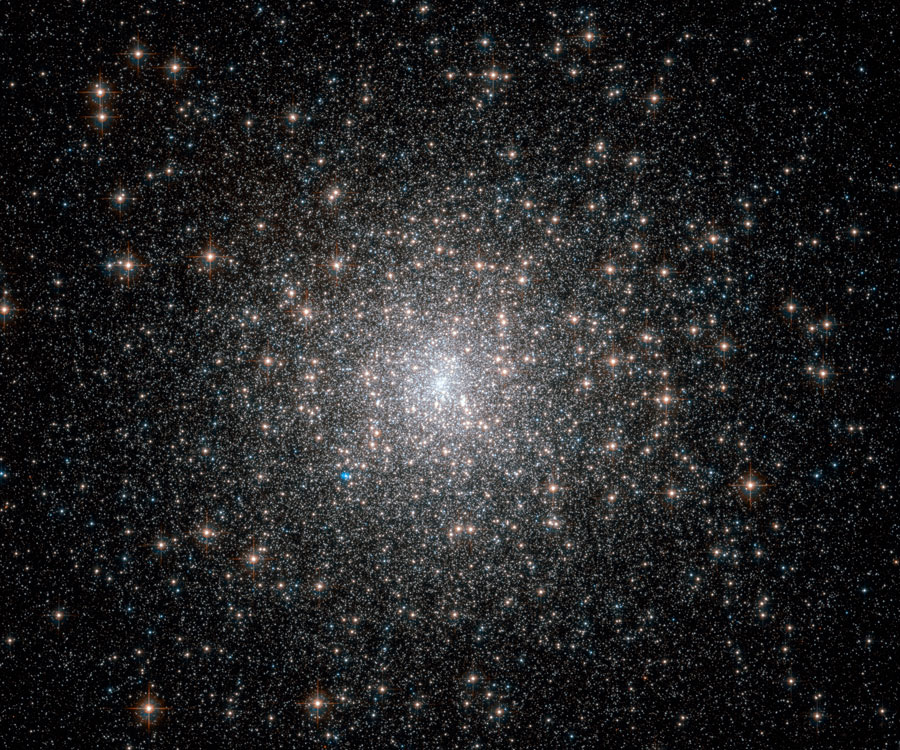
\includegraphics[width=12cm]{images/m15.jpg}
\caption[M15 Globular Cluster]{Globular Cluster M15, taken by the Hubble Space Telescope with an exposition time of 900 seconds. Image by NASA}
\end{figure}

Let's discuss in further the details of these systems.

\subsection{Basics}

A Globular Cluster is a compact, gravitationally bound group of hundreds of thousands to several million stars that are themselves gravitationally bound to galaxies. They have comparable ages to their associated galaxies which is an encouraging characteristic to study them as they could provide valuable information about the formation and evolution of their host galaxies.

Their star populations are uniformly old, although different stellar populations are found as we improve our measurements and observations. Globular clusters are devoid of gas so that pretty much no new stars form in them. The stars at the centre of a globular cluster are much more densely packed than the stars in other parts of the galaxy.

Globular clusters revolve about the nucleus of a galaxy on orbits of high eccentricity and high inclination to the galactic plane. About a third of globular clusters are concentrated around the galactic center. A typical cluster has a period of revolution around the order of $ 10^{8} $ years. A cluster spends most of its time far from the center of a galaxy, and so most of them can, and have been discovered in the spaces between galaxies. 

Due to clusters moving in various orbits in the Galaxy, they are bound together with gravitational forces that are stronger than the disrupting forces exerted on it by the Galaxy or other nearby stars, and this results in an added condition for the stability of a cluster.

The spherical shape of these systems is due to the reached stability that they can acquire over time. To ensure the stability of an isolated cluster, the average speed of its individual stars must not exceed the escape velocity from the cluster. If this occurred, the stars would escape into space, and the cluster would dissipate. If the stellar velocities are low enough to satisfy this condition, then the cluster is gravitationally bound, i.e. the force of gravity is strong enough to keep the member stars from escaping.

Another factor in the stability of clusters is size; the smaller and more compact the cluster, the greater its own gravitational binding force compared with the disrupting forces, and the more chance it has to survive to old age.

Because globular clusters are highly compact systems, they are consequently very stable, and so most globular clusters will probably maintain their identity almost indefinitely. But even these clusters lose some stars, especially if they have a low mass. This is due to there always being a few stars in a cluster that move faster than the cluster's average speed.

When a star escapes, it carries with it energy, removing this energy from the cluster as a whole. This eventually results in the cluster developing a tightly bound core surrounded by a rarefied halo of stars as we can see in the following images of Globular Clusters:

\begin{figure}[H]
\centering
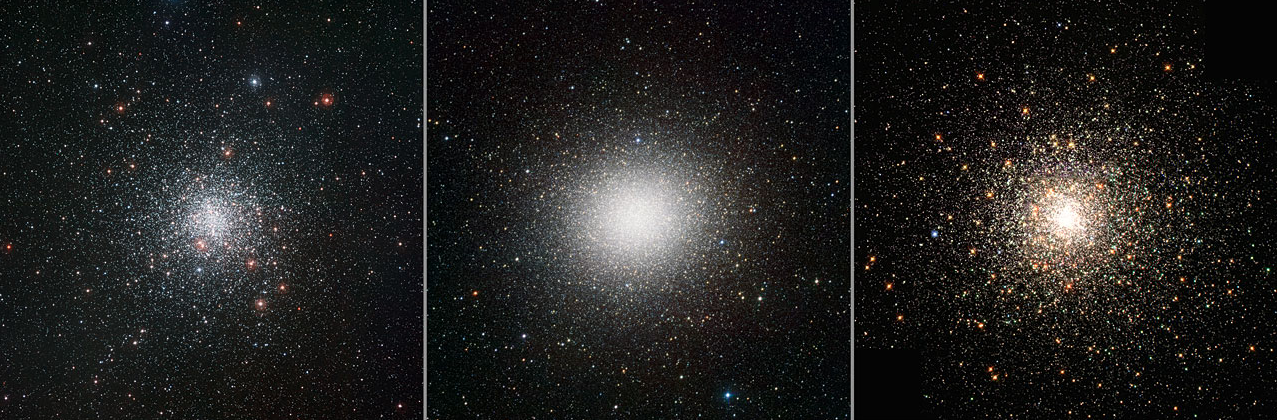
\includegraphics[width=14.5cm]{images/3_gcs.png}
\caption[ESO and Hubble images of Globular Clusters]{Globular Clusters taken by ESO and the HST. From left to right: M4 (ESO), Omega Cen (ESO) and M80 (Hubble). Image from the Hubble Space Telescope database.}
\end{figure}

In the dense core of a cluster, the stars occasionally collide, and some of the debris eventually coalesces. Predictions indicate that this dynamical evolution could lead to the development of a large Black Hole at the cluster's center. At the same time, a few stars in the outer parts of the cluster would continue to escape. The escape rate and dynamical evolution for the rich globular clusters are so slow that the clusters can easily survive for many billions of years, remaining mostly unchanged.

Observations and mass models of these structures show that the average star density in a Globular Cluster is about 0.4 stars per cubic parsec. In the dense center of the cluster, the star density can increase from 100 to 1000 per cubic parsec, as we shall discuss in another section. However, even in the center of clusters, there is still plenty of space between the stars.

In order to understand how dense Globular Clusters can be, we may think of a clear example like Proxima Centauri, which is 4.2 light-years, or about 1.3 parsecs from Earth. Thus, if we were able to draw a sphere around the Sun with a radius of 1.3 parsecs, it would only contain 2 stars: the Sun and Proxima Centauri. But if you were to draw this same sphere in the center of the globular cluster M13, it would contain approximately 10,000 stars.

To summarize and compare some of the main characteristics we just mentioned about globular clusters with other stellar systems let's see the following table:

\begin{table}[H]
\begin{tabular}{| c | c | c | c |}
\hline
\textbf{Characteristic}              & \textbf{Open Custers} & \textbf{OB Associations} & \textbf{Globular Clusters}  \\
\hline
Diameter $ (pc) $ & $<10$ & $30-200$ & $20-100$ \\ \hline
Number of Stars & $50-1000$ & $10-100$ & $10^{4}-10^{6}$ \\ \hline
Mass ($M_{\odot}$) & $100-1000$ & $100-1000$ & $10^{4}-10^{6}$ \\ \hline
Density ($M_{\odot}/pc^{3})$ & $0.1-10$ & $<0.01$ & $0.5-1000$ \\ \hline
Shape & Irregular & Irregular & Spherical \\ \hline
Color (Common) & Red or Blue & Blue & Red \\ \hline
Metallicity & High & High & Low \\ \hline
Location & Disk of Galaxy & Disk of Galaxy & Halo of Galaxy \\
\hline
\end{tabular}
\caption[Summary chart of Star Clusters]{Summary chart of Star Clusters, taken from  http://astronomyonline.org}
\end{table}

\subsection{Formation and evolution}

The formation of Globular Clusters is not well understood yet, and we only have crude ideas of their typical states right after they have reached the dynamical equilibrium.

As it was mentioned in the introduction, two main broad types of possibilities have been considered to explain the very first processes that created these structures. The first one suggests that in the early universe the first structures that came to exist were globular clusters by Jeans Fragmentation. One of the main contributions to this possibility was given by Peebles \& Dicke (1968) who first pointed out that globular clusters might have formed even before the collapse of the protogalaxy, noting the fact that the baryonic Jeans mass right after decoupling is about the size of a Globular Cluster. Although their possibility is in concordance with the current scenario of galaxy formation in which galaxies are formed inside the deepest regions of the gravitational potential well provided by dark matter halos, there are still problems of this theory, for example, it cannot explain why there are so few intergalactic globular clusters and why the properties of globular clusters are correlated with their host galaxies.

Another problem with this theory is some observational results like the ones found by Odenkirchen et al. (2003) who found tidal tails surrounding globular clusters. This is not expected if globular clusters form and reside inside extended dark matter halos that would keep the stability and thus avoiding the creation of these tidal tails.

The second possibility suggests that the formation of Globular clusters was a response to thermal instabilities present in large hot halos of massive galaxies full of gas. In their model, cold dense clouds condense out of hot and tenuous background to form as progenitors of globular clusters. This idea corresponds to the late-forming theory Globular Clusters that could be in accordance with the present observational properties of Globular Clusters like their characteristic metallicity, but it has proven difficulties to justify the assumed thermal behaviour of the cluster-forming gas clouds. Also, there are observations that suggest that very low mass galaxies, not massive enough to host a hot gaseous halo, may also have their own globular clusters.

Many theories on Globular Cluster formation assume a smooth and rapid collapse of the protogalaxy (Eggen, Lynden-Bell, \& Sandage 1962) but some other authors (Searle \& Zinn 1978) state that the early Galactic environment migth have been much more chaotic and violent.

Murray \& Lin (1992) have argued that self-gravitating clouds are unstable to fragmentations and spontaneous star formation so that globular clusters must form from sub-Jeans mass clouds. In subsequent work Murray et al. (1993) have shown that only clouds in a limited mass range ($10^{4}M_\odot\lesssim M\lesssim 10^{6}M_\odot$) can survive both the Kelvin-Helmholtz  instability and the thermal instability which does not lead to bound clusters. Clouds within the critical mass range will form globular clusters if they are induced into cooling and collapse by collisions of sufficient velocity.

Mathews \& Schramm proposed a schematic merger model for the formation of the halo and chemical evolution of the Galaxy in which the protogalaxy forms by mergers of small subgalactic gas clouds. This merger model, as discussed by Lee, Schramm \& Mathews 1994 could also be a possible scenario for Globular Clusters formation. 

Moving on to the evolution of these systems, we note that our current observations and modelling give us good results after the equilibrium has been reached, in this context, there must be mentioned that the mechanism that drives the system to stability is relaxation. This proccess pretty much erases the cluster's memory of it's initial state so the results for gravitational stable systems can be reached using a wide range of initial conditions.

Since the relaxation time is inversely proportional to density evolution due to relaxation proceeds most rapidly in the dense central regions of the clusters. Within this central region that is relaxed, the distribution function $f$ and the density distribution should be approximate to a isothermal distribution, this means that the distribution function must be approximately Maxwellian at energies well bellow the escape energy. We asume that in the outer parts of the clusters the relaxation time is long and encounters have relatively little effect.

Other important characteristic of their evolution is they lose mass from stellar evolution: Our stellar evolution theories show us that stars often eject mass from their surfaces near the ends of their lives. For the mass-losing stars inside globular clusters, the ejected mass is likely to escape the cluster, either because the ejection velocity exceeds the escape speed from the cluster or because it interacts with the galactic gas when the cluster is passing throw the disk. So we conclude that the clusters lose mass as stars evolve. It must be mentioned that the evolution timescale of a typical population of stars is usually much longer than the crossing time in the cluster.

The mass lost by a cluster due to stellar evolution depends on the initial mass function  which specifies the distribution of masses of stars just after they have formed and the initial-final mass function. 

Now, when we talk about the evolution of the Globular Clusters, we must see how the mass distribution evolves over time. the evolution of the mass distribution in an isolated cluster, that began as a Plummer model (that we shall introduce in the following section) is shown in the next figure:

\begin{figure}[H]
\centering
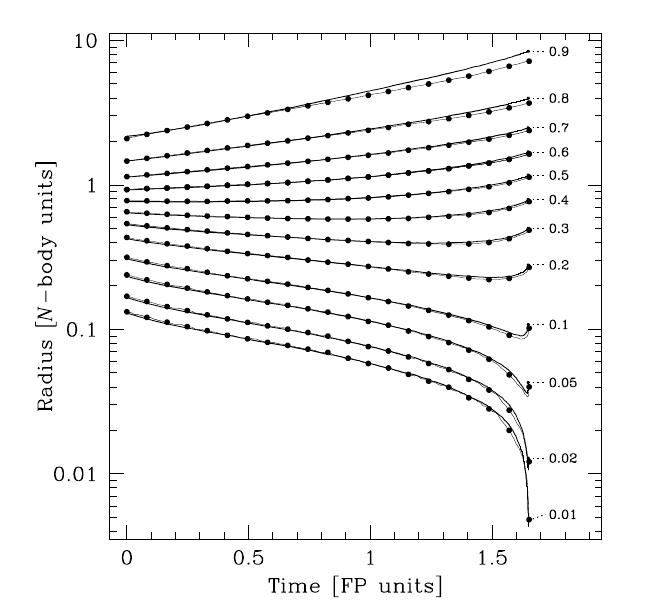
\includegraphics[width=12cm]{images/core_collapse.png}
\caption[Evolution of an ergodic Plummer model over time]{Evolution of an ergodic Plummer model, according to an orbit-averaged Monte-Carlo solution of the Fokker Planck equation with $3\times10^{5}$ superstars (heavy solid lines) and an N-body simulation with $65536$ superstars (dots, connected by solid lines). From Freigat, Rasio, \& Baumgardt (2006)}
\end{figure}

As we can see above, the outer half of the cluster expands, mainly due to the gradual growth of the halo as stars in the core diffuse towards the escape energy. But most importantly, we can see that the center contracts, this process is known as \textbf{core collapse} and it leads to a dramatic growth in the central density that may indicate the existence of an apparent singularity in the central density.

By solving the orbit-averaged Fokker-Planck equation for an isolated, spherical cluster (without binaries) and starting from a Plummer model, Takahashi (1995) found a more accurate calculation of core collapse. His calculations allow greater dynamic range than Monte Carlo or N-body methods. His results show that as the cluster evolves, the core radius shrinks  and the central density grows. Outside the core, the density profile approaches a power law $\rho\varpropto r^{-2.23}$.

Another interesting result regarding the direct solutinos of the orbit-avergaed Fokker Planck equations is the behaviour of the anisotropy parameter $\beta=1-\overline{v_{\theta}^{2}}/\overline{v_{r}^{2}}$ as we can see in the following figure:

\begin{figure}[H]
\centering
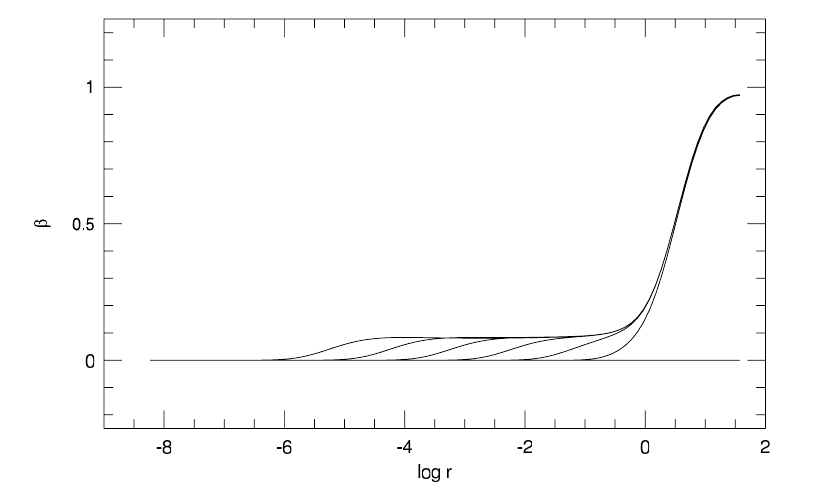
\includegraphics[width=12cm]{images/anisotropy_core_collapse.png}
\caption[Evolution of the velocity anisotropy parameter]{The evolution of the velocity anisotropy parameter for an orbit-averaged Fokker Planck calculation of core collapse. From Takahashi (1995)}
\end{figure}

At large radii, the anisotropy parameter (that indicates the tendency of the system to have or not preferred directions) tends to unity ($\beta\simeq1$), and that indicates that the orbits are nearly radial, at the smalest radii, inside the shrinking core, we have $\beta\simeq0$, which indicates that the velocity distribution is isotropic. We note that in the radius range in which the density profile in the top panel is a power law, there is a constant small radial anisotropy of $\beta\simeq0.08$ or  $\overline{v_{\theta}^{2}}/\overline{v_{r}^{2}}\simeq0.92$

Regarding the late interactions and accretion processes, we note that although our Galaxy has evidently not experienced any further major accretion events capable of disrupting the disk, it is possible that minor accretion events affecting only the halo and not the disk have continued to occur (Navarro, Frenk, \& White 1994), but their net effect on the GC's dynamics and stability is the context of cosmology is very low.

The evolution process for these systems are so long that this fit entirely in the context of Cosmology. Most of the clusters whose masses are larger than $10^{5}M\odot$ have lifetimes longer than the Hubble time.

\subsection{Observational Properties}

Globular clusters were once thought to consist of a single population of stars that all formed together. However, research has since shown that many of the Milky Way's globular clusters had far more complex formation histories and are made up of at least two distinct populations of stars.

A way of analysing the stellar populations in Globular Clusters is to use Colour-Magnitude diagrams. A colour-magnitude diagram is a plot of the apparent magnitudes of the stars in a cluster against their colour indices. Globular Clusters nearly all have very similar colour-magnitude diagrams.

This diagram for a typical globular cluster looks very different than that of an open cluster. There are no Main Sequence stars of types OBAF, but there are many red giants. The brightest stars in a globular cluster are those at the tip of the red giant branch in the color-magnitude diagram, which explains the red appearance of the bright stars in color images of the clusters. You can also see stars populating the horizontal branch (and also why it is called the horizontal branch), the asymptotic giant branch, and even some stars that have colors and magnitudes of F stars, but far fewer than the G stars just below and to the right of them on the Main Sequence. As we can see in the following figure:

\begin{figure}[H]
\centering
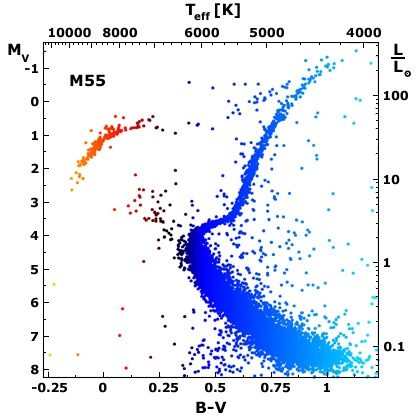
\includegraphics[width=10cm]{images/m55_diagram.jpg}
\caption[Color Magnitude diagram of M55]{Color Magnitude diagram of M55. Image by NASA}
\end{figure}
 
Of these populations, around half the stars are a single generation of normal stars that were thought to form first, and the other half form a second generation of stars, which are polluted with different chemical elements. In particular, the polluted stars contain up to 50–100 times more nitrogen than the first generation of stars.

The proportion of polluted stars found in the Milky Way's globular clusters is much higher than astronomers expected, suggesting that a large chunk of the first-generation star population is missing. A leading explanation for this is that the clusters once contained many more stars, but a large fraction of the first-generation stars were ejected from the cluster at some time in its past.

An interesting plot relating the age of the Globular Clusters to their metallicity is shown in the following figure:

\begin{figure}[H]
\centering
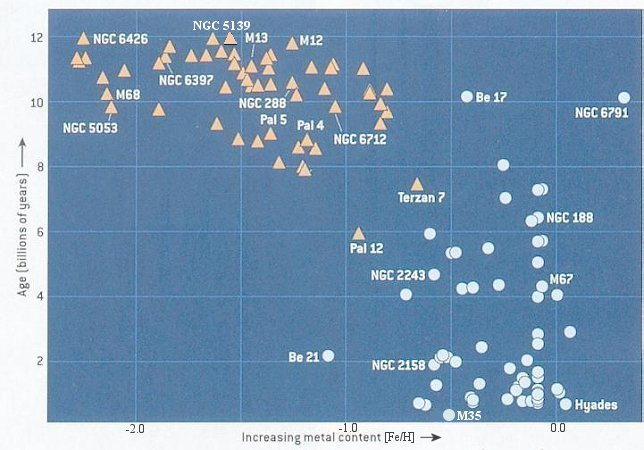
\includegraphics[width=10cm]{images/metallicity_gcs.jpg}
\caption[Age vs Metallicity for some Globular Clusters]{Age estimations vs metallicity of Open (circles) and Globular (triangles) Clusters. Taken from https://universe-review.ca}
\end{figure}

Before now, we didn't know whether globular clusters in smaller galaxies had multiple generations or not, but our observations show clearly that they do. This finding means that a leading theory on how these mixed-generation globular clusters formed cannot be correct, and astronomers will have to think once more about how these mysterious objects in the Milky Way and further afield came to exist.

The other fundamental observational procedures to study GC's are Radial velocity measurements that have revealed that most Globular Clusters are moving in highly excentric elliptical orbits that take them far outside the Milky Way; they form a halo of roughly spherical shape which is highly concentrated to the Galactic Center, but reaches out to a distance of several 100,000 light years, much more than the dimension of the Galaxy's disk. As they don't participate in the Galaxy's disk rotation, they can have high relative velocities of several 100 km/sec with respect to our solar system; this is what shows up in the radial velocity measurements. Ninkovic (1983) has estimated eccentricities of globular cluster orbits.

We can visualize their orbits in the following figure:

\begin{figure}[H]
\centering
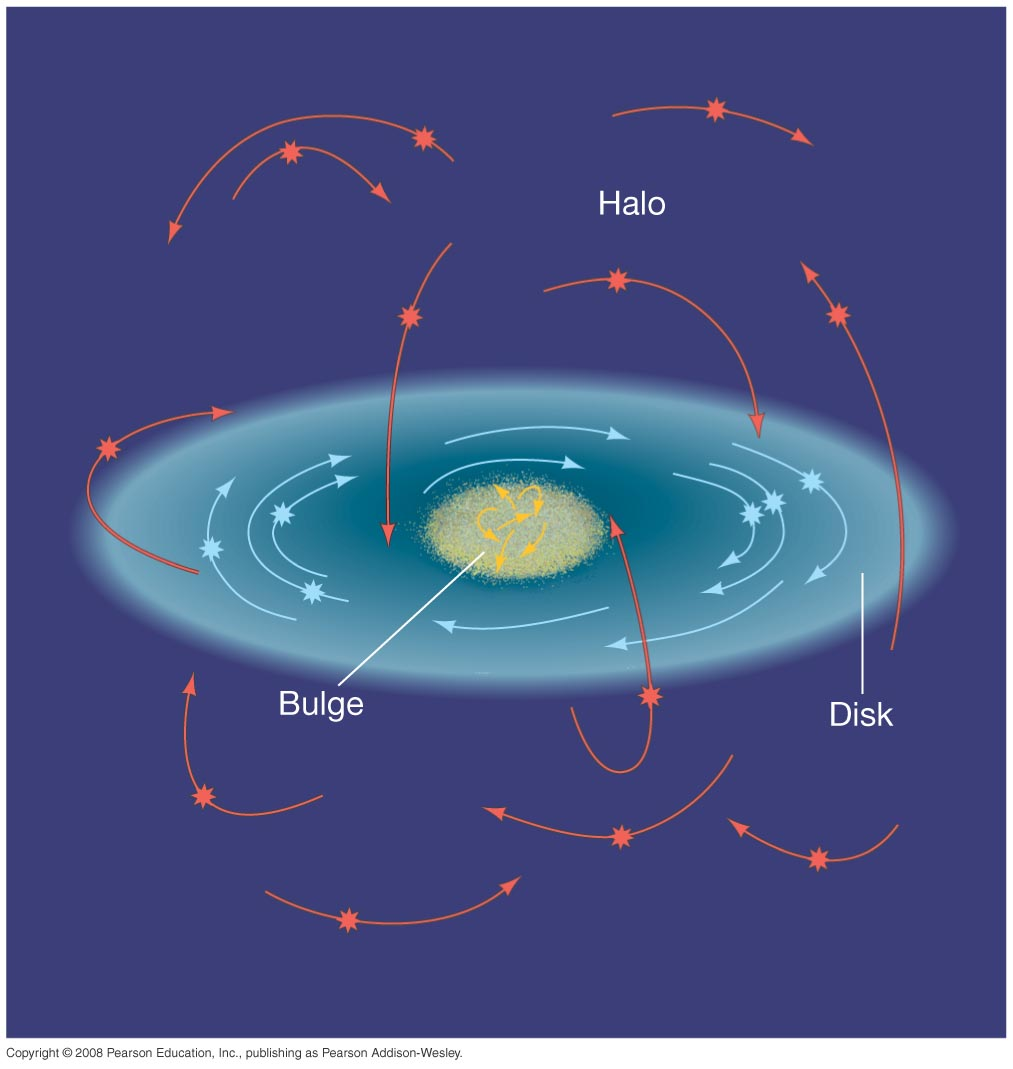
\includegraphics[width=10cm]{images/orbits_gcs.jpg}
\caption[Illustration of the orbits of Globular Clusters around a spiral galaxy]{Illustration of the orbits of some Globular Cluster in a spiral galaxy like the Milky Way. Picture from the Oregon University webpage}
\end{figure}

To determine the physical orbits of globular clusters, it is required to know their proper motions in addition to the radial velocities. Cudworth and Hanson (1993) undertook some first rough determinations of proper motions with respect to background galaxies. From these and similar measurements, Van den Bergh (1995) estimated perigalactic distances, and Dauphole et.al. (1996) calculated first approximate orbits. Much more acurate data for proper motions became only available from astrometrical data obtained with ESA's Hipparcos satellite in 1997, from which space motions (Geffert et.al. 1997) and approximate orbits (Brosche et.al. 1997) could be determined.

\section{Mass models and Dynamics}

In order to get into the physical discussions about the stability and modelling of globular clusters, we need to understand first the basics of potential theory, and more specifically the potential theory of spherical systems. The next step is to discuss the physical implications behind these models so that the mass modelling can be made. The last but most important part is to discuss the criteria regarding the mathematical treatment of the dynamics of these systems in the context of the collisionless Boltzmann equation and the approximations to the solutions of the Jeans equations that will be used for the fitting of the observational data to do the final modelling.

\subsection{Potential Theory of Spherical Systems}

Our discussions about Potential Theory for large stellar systems will be studied using the simplifications given by the spherical symmetry of globular clusters. We first introduce some of the most important theorems for calculating the gravitational potential of an spherically symmetric distribution of matter provided by Newton, these theorems are physically related to Gauss theorem and may be proved using simple geometric assumptions or using a more precise results from vectorial calculus.

\textbf{Newton's first theorem} states that a body that is inside a spherical shell of matter experiences no net gravitational force from that shell. 

\textbf{Newton's second theorem} states that the gravitational force on a body that lies outside a sphericall shell of matter is the same as it would be if all the shell's matter were concentrated into a point at its center. 

It follows from Newton's theorems that the gravitational attraction of a spherical density distribution $\rho(r')$ on a unit mass at radius $r$ is entirely determined by the mass interior to $r$:

\begin{equation}
\textbf{F}(r)=-\frac{GM(r)}{r^{2}}\hat{\textbf{e}}_{r}
\end{equation}

Where the mass as a function of the radius is

\begin{equation}
M(r)=4\pi\int_{0}^{r}dr'r'^{2}\rho(r')
\end{equation}

We can consider that the total gravitational potential of the spherical system is the sum of the potentials given by spherical shells of a diferential mass $dM(r)=4\pi\rho(r)r^{2}dr$. This way, we may calculate the gravitational potential at $\textbf{r}$ generated by a spherically symmetruc density distribution $\rho(\textbf{r}'$ by adding the contributions to the potential produced by shells with $r'<r$, and with $r'>r$. Thus we obtain:

\begin{equation}
	\begin{aligned}	
	\Phi(r) &= -\frac{G}{r}\int_{0}^{r}dM(r')-G\int_{r}^{\infty}\frac{dM(r')} {r'}\\      &= -4\pi G\left[\frac{1}{r}\int_{0}^{r}dr'r'^{2}\rho(r')+\int_{r}^{\infty}dr'r'\rho(r')\right]
	\end{aligned}
\end{equation} 

We note an important property of a spherical matter distribution regarding its circular speed $v_{c}(r)$, defined to be the speed of a particle of negligible mass in a circular orbit at radius $r$. We may evaluate $v_{c}$ by equating the gravitational attraction $|\textbf{F}|$  to the centripetal acceleration ${v_{2}}^{2}/r$:

\begin{equation}
v_{c}^{2}=r|\textbf{F}|=r\frac{d\Phi}{dr}=\frac{GM(r)}{r}
\end{equation}

We may also note that the \textbf{escape speed} $v_{e}$ in terms of the gravitational potential is:

\begin{equation}
v_{e}(r)\equiv\sqrt{2|\Phi(r)|}
\end{equation}

The \textbf{potential energy of spherical systems}  comes from a very general equation, also in terms of the potential:

\begin{equation}
W=-\int d^{3}x\rho x\cdot\nabla\Phi
\end{equation}

By substituting equation (2.1) and integrating over all directions of \textbf{r} we get:

\begin{equation}
W=-4\pi G\int_{0}^{\infty}drr\rho(r)M(r)
\end{equation}

The potential energy tensor of a spherical body is \textbf{diagonal} i.e it is isotropic, and has the form:

\begin{equation}
W_{jk}={{1}\over{3}}W\delta_{jk}
\end{equation}

Once we have the general results for the potential of spherical distributions we can move on to study special cases, let's study potential-density pairs that would best fit for Globular Clusters.

The simplest model is the \textbf{homogeneous sphere} of radius $a$, characterized by the gravitational radius $r_{g}\equiv GM^{2}/|W|$, with $r_{g}=\frac{5}{3}a$, for which the gravitational potential is:

\begin{equation}
\Phi(r) = \left\lbrace
\begin{array}{ll}
-2\pi G\rho\left(a^{2}-\frac{1}{3}r^{2}\right) & (r<a)\\
-\frac{4\pi G\rho a^{3}}{3r} & (r>a)
\end{array}
\right.
\end{equation} 

For spherical systems, the density is roughly constant near the center, and falls to zero at large radii. A potential of a system of this type would be proportional to $r^{2} + constant$ at small radii and to $r^{-1}$ at large radii. The \textbf{Plummer Model} is a simple potential with these properties and it it of the form:

\begin{equation}
\Phi=-\frac{GM}{\sqrt{r^{2}+b^{2}}}
\end{equation}

What characterises this model to a simple homogeneous sphere model is the linear scale that generates the potential, which is called the \textbf{Plummer scale length} $b$ while $M$ represents the total mass of the system. From this potential, using spherical coordinates we can calculate $\nabla^{2}$:

\begin{equation}
\nabla^{2}\Phi=\frac{1}{r^{2}}\frac{d}{dr}\left(r^{2}\frac{d\Phi}{dr}\right)=\frac{3GMb^{2}}{\left(r^{2}+b^{2}\right)^{5/2}}
\end{equation}

And from $\nabla^{2}\Phi=4\pi G\rho$ (\textbf{Poisson's equation}) the corresponding density to the potential:

\begin{equation}
\rho(r)=\frac{3M}{4\pi b^{3}}\left(1+\frac{r^{2}}{b^{2}}\right)^{-5/2}
\end{equation}

And finally the potential energy of a Plummer model is:

\begin{equation}
W=-\frac{3\pi GM^{2}}{32b}
\end{equation}

In 1911 Plummer used this potential-density pair to fit observations of Globular Clusters since it gets rid if the indetermination that would arise if we didn't include the Plummer scale length.

Another useful model is given by the \textbf{Isochrone Potential}, that gives analytic orbits to all the stars orbiting the system (For a Plummer potential the position of a star orbiting the system cannot be given in terms of elementary functions). This model is of the form:

\begin{equation}
\Phi(r)=-\frac{GM}{b+\sqrt{b^{2}+r^{2}}}
\end{equation}

By Poisson's equation the density associated with the isochrone potential is:

\begin{equation}
\rho(r)=\frac{1}{4\pi G}\frac{1}{r^{2}}\frac{d}{dr}\left(r^{2}\frac{d\Phi}{dr}\right)=M\left[\frac{3\left(b+a\right)a^{2}-r^{2}(b^{2}+3a)}{4\pi(b+a)^{3}a^{3}}\right]
\end{equation}

So that in the extreme cases the isochrone potential yields:

\begin{equation}
\rho(r) = \left\lbrace
\begin{array}{ll}
\frac{3M}{16\pi b^{3}} & (r=0)\\
\frac{bM}{2\pi r^{4}} & (r\gg b)
\end{array}
\right.
\end{equation} 

As a very useful approximation, we can work with \textbf{Two-power density models}. First, we note that the luminosity density of many elliptical galaxies can be approximated as a power law in radius at both the largest and smallest observable radii, with a smooth transition between these power laws at intermediate radii. Some numerical simulations of the clustering of dark matter particles suggest that the mass density within a dark halo has a similar structure. This is the reason for which much attention has been given to models with a density of the form:

\begin{equation}
\rho(r)=\frac{\rho_{0}}{\left(r/a\right)^{\alpha}\left(1+r/a\right)^{\beta-\alpha}}
\end{equation}

Dark matter halos are often modelled by the above equation with $\beta\simeq3$ and $\alpha$ in the range $(1,1.5)$. Dehnen models are the solutions for $\beta =4$ that have simple analytic properties. But we may discuss some specific results summarized in the following table:

\begin{table}[H]
\begin{center}
  \begin{tabular*}{0.35\textwidth}{@{\extracolsep{\fill} } c  c  c }
    \hline
    \textbf{Model} & $\alpha $ & $\beta $ \\ \hline
    Hernquist (1990) & 1 & 4 \\
    Jaffe (1983) & 2 & 4 \\
    NFW (1995) & 1 & 3 \\
    \hline
  \end{tabular*}
\end{center} 
\caption[Two power density potentials]{Two-power densitiy potentials given by the different values of $\alpha$ and $\beta$}
\end{table}

Navarro, Frenk, \& White (1996) showed that the values taken by the free parameters $\alpha$ and $\beta$ for the halos that formed in their simulations were strongly correlated, so the halos were essentially members of a one-parameter family. 

According to equation (2.17) the mass inside the radius $r$ is:

\begin{equation}
M(r)=4\pi \rho_{0}a^{3}\int_{0}^{r/a}ds\frac{s^{2-\alpha}}{(1+s)^{\beta-\alpha}}
\end{equation}

For the important cases we discuss, the mass is

\begin{equation}
M(r) = 4\pi \rho_{0}a^{3} \times \left\lbrace
\begin{array}{lll}
\frac{r/a}{1+r/a} & \text{for a Jaffe model}\\
\frac{(r/a)^{2}}{2(1+r/a)^{2}} & \text{for a Hernquist model}\\
ln(1+r/a)-\frac{r/a}{1+r/a} & \text{for a NFW model}
\end{array}
\right.
\end{equation} 

We can directly integrate the mass to get the potential for the three discussed models:

\begin{equation}
\Phi(r) = -4\pi G\rho_{0}a^{2} \times \left\lbrace
\begin{array}{lll}
ln(1+r/a) & \text{for a Jaffe model}\\
\frac{1}{2(1+r/a)} & \text{for a Hernquist model}\\
\frac{ln(1+r/a)}{r/a} & \text{for a NFW model}
\end{array}
\right.
\end{equation} 

From the above equations, and taking into account the potential energy for each model, it can be proved that the Jaffe and Hernquist models have gravitational radii $r_{r}=2a$ and $6a$ respectively, while for the NFW model $r_{g}$ is undefined. The circular speed, given by these potentials for each model is shown in the following figure: 

\begin{figure}[H]
\centering
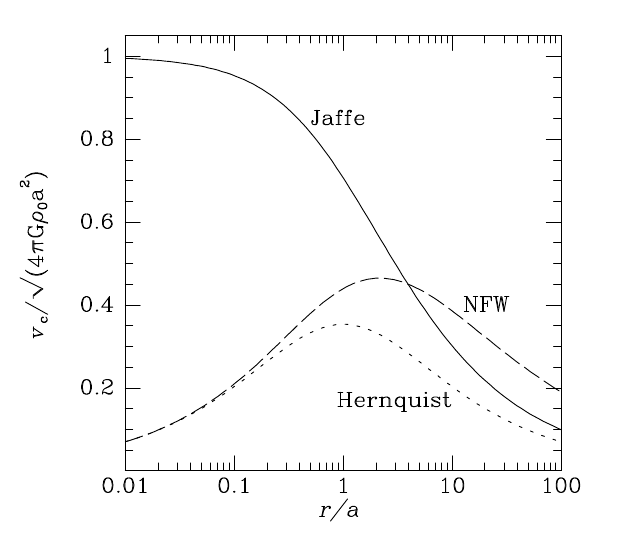
\includegraphics[width=10cm]{images/circular_velocity_vs_radius.png}
\caption[Circular speed vs radius for the Jaffe, Hernquist, and NFW models]{Circular speed vs radius for the models of Jaffe, Hernquist and NFW, taken from Binney \& Tremaine, Galactic Dynamics 2nd edition.}
\end{figure}

The next step in the analysis of the dynamics and stability of Globular Clusters is to understand the physics of spherical distribution of systems and how the solutions for their dynamics can be easily reached. As we shall see, a good consideration for the simplification of the mathematical treatment of Globular Clusters (with good physical reasons) is that these systems are not collisional.

\subsection{Collisionless Systems}

The problem of modelling the structure and dynamics of Globular Clusters is not trivial whatsoever. Several assumptions and physical approaches need to be made to simplify the problem and reach results that fit the observational data. One of the main assumptions is that the stellar systems that we will study are \textbf{collisionless}. This assumption not only reduces the problem of determining the functional form of the position and velocities of the stars but also has strong physical reasons that must be mentioned.

In the context of stellar systems, collision refers to any interaction between individual particles, such as direct encounters, gravitational assistance, sudden disruption of the orbit, or any interaction that changes the stars orbit in a significant way. That the system is collisionless means that it is a system in which the interaction cross-section between particles (stars in this case) is so low that collisions between particles have no significant effect on the system, and that the dominant component of the dynamics is the potential well produced by the system as a whole.  

One of the other approximations we make is that the orbits of stars in the system can be determined by assuming that the mass of the Globular Cluster is distributed smoothly in space, rather than concentrated in certain positions as point masses. The true orbits deviate significantly from this approximated model, but in systems with more than a few thousand stars like a globular cluster (that can easily reach hundreds of thousands or millions of stars), the deviation is small for a time smaller than the relaxation time $t_{relax}$ that is much larger than the crossing time $t_{cross}$.

relaxation usually means the return of a perturbed system into equilibrium

Stellar encounters lead to dynamical relaxation, wheby
the system is in a thermal equilibrium. 

Define this as
the relaxation time - time required for the star to lose all memory
of its initial orbit.

crossing time:

\begin{equation}
t_{cross}=\frac{R}{V}=\frac{6ln(N)}{N}v^{2}
\end{equation}

The relaxation time in terms of the crossing time is:

\begin{equation}
t_{relax}=\frac{N}{6ln(N)}t_{cr}
\end{equation}

\begin{equation}
\dfrac{df}{dt}=0
\end{equation}

\subsection{Dynamics}

(Collisionless Boltzmann equation, Distribution Function, Jeans equations)

\begin{equation}
\frac{df}{dt}=0
\end{equation}

\begin{equation}
\frac{\partial f}{\partial t}+\sum_{i=1}^{3}\frac{\partial f}{\partial x_{i}}\dot{x_{i}}+\sum_{i=1}^{3}\frac{\partial f}{\partial v_{i}}\dot{v_{i}}=0
\end{equation}


\begin{equation}
\dot{v_{i}}=-\frac{\partial\phi}{\partial x_{i}}
\end{equation}

\begin{equation}
\frac{\partial f}{\partial t}+\nabla f\cdot\vec{v}+\frac{\partial f}{\partial\overrightarrow{v}}\cdot\nabla\phi=0
\end{equation}

Moment of order $j$ of the distribution $f$

\begin{equation}
\overline{x^{j}}=\frac{\int x^{j}fdx}{fdx}
\end{equation}

velocity dispersion tensor:

\begin{equation}
\sigma_{ij}^{2}=\overline{v_{i}v_{j}}-\overline{v_{i}}\:\overline{v_{j}}
\end{equation}

Anisotropy parameter:

\begin{equation}
\beta=1-\frac{\left(\sigma_{\theta}^{2}+\sigma_{\phi}^{2}\right)}{2\sigma_{r}^{2}}
\end{equation}

When $\beta=1$ total anisotropy

\section{Scenario and Observations}

The first globular cluster discovered, but then taken for a nebula, was M22 in Sagittarius, which was probably discovered by Abraham Ihle in 1665. This discovery was followed by that of southern Omega Centauri (NGC 5139) by Edmond Halley on his 1677 journey to St. Helena. This "nebula" had been known but classified as star since ancient times. Next followed the discovery of M5 in Serpens Caput by Gottfried Kirch in 1702, and that of M13 in Hercules, again by Halley, in 1714. De Chéseaux's list of (21) nebulae of 1746 contains, in addition, two new globular clusters, M71 and M4, while Jean-Dominique Maraldi discovered M15 and M2 in September of this year (1746). Guillaume Legentil possibly or probably discovered NGC 6712 in 1749. Nicholas Louis de Lacaille's catalog of (42) southern "nebula" of 1751-52 contains 8 globular clusters (among them 5 new ones), while Messier's catalog of 110 objects contains a total of 29 globulars, 20 of them new discoveries. Charles Messier was the first to resolve one globular cluster, M4, but still referred to the other 28 of these objects in his catalog as "round nebulae." Thus, in summer 1782, before William Herschel started his comprehensive deep sky survey with large telescopes, there were 34 globular clusters known. Herschel himself discovered 36 new globulars, bringing the number of known globulars to 70. He was the first to resolve virtually all of them into stars, and coined the term "globular cluster" in the discussion adjacent to his second catalog of 1000 deepsky objects (1789).


there is  widesprea belief that globular clusters cannot contain large amounts of dark matter, because of the Virial Theorem. This theorem relates the velocity dispersion $ \sigma $ at the center of the cluster to the total mass $M_{t}$ and to the half-mass radius $r_{h}$ of the system. For a one component globular cluster, that relation may be expresed as:

\begin{equation}
\left\langle \sigma^{2}\right\rangle \approx0.4\frac{GM_{t}}{r_{h}}
\end{equation}

However, if a dark component is also present, in the form of low-mass objects for example, the virial theorem must be modified to:

\begin{equation}
\sum_{i}M_{t}(i)\left\langle \sigma^{2}\right\rangle _{i}=E_{p}
\end{equation}

where the index $i$ refers to the different stellar species, and $E_{p}$ is the potential energy of the cluster.

\section{Simulations}

Efforts are under way by several groups to produce more realistic simulations that properly include the effects
of star formation, but the existing results suggest that the first star formation may occur in gas that has become highly condensed at the centers of the first dark-matter halos to form; even though such systems may not closely resemble most present-day galaxies, they may still be of interest as the possible birth sites
of globular clusters, as will be discussed further below. The most realistic simulations of the formation of a spiral galaxy like our own have been made by Katz (1992) and Steinmetz \& Muller (1994, 1995), who have simulated the evolution of a spherical galaxy-sized piece of a standard "cold dark matter" universe which is arbitrarily given the appropriate amount of angular momentum. The results show an initial chaotic stage during which mergers between clumps build up a dark halo and a stellar spheroid, followed by a period during which the remaining gas organizes itself into a disk. During the initial chaotic stage several small satellites are formed by the condensation of gas in peripheral dark-matter clumps, and these satellites may survive for a few
orbits before being disrupted and merged into the forming galaxy. It is plausible that such small satellites could be the birth sites of globular clusters, as in the hypothesis of Searle (1977) and Searle \& Zinn (1978) that the globular clusters in the outer halo of our Galaxy were formed in protogalactic ‘fragments’ which
survived for a time as independent star-forming systems before being merged to build up the halo

In several earlier reviews of globular cluster chronology, it was concluded that the globular clusters in our Galaxy are not all coeval and that age differences of several Gyr exist in at least a few well-studied cases (e.g., Larson 1990a, 1992b). This conclusion still appears to be valid, and it is supported by the most recent discussion of this subject by Chaboyer, Demarque, \& Sarajedini (1996), which is based on new age estimates for 43 globular clusters

\begin{figure}[H]
\centering
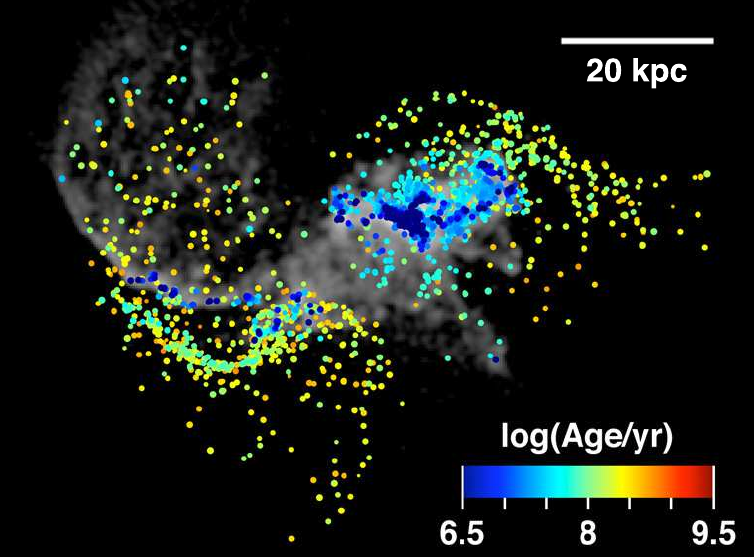
\includegraphics[width=10cm]{images/merger.png}
\caption[Galaxy merger model 1m11 from Kruijssen et al. (2012b)]{Snapshot of galaxy merger model 1m11 from Kruijssen et al. (2012b), which includes a sub-grid model for the formation and evolution of the stellar cluster population. SHown is a merger of two Milky Way-mass galaxies at the time of their first encounter. Coloured dots represent stellar clusters, clour-coded by their ages as indicated by the legend. The grey scale indicates the gas surface density. The snapshot shows how intermediate-age clusters are escaping into the halo, whereas those clusters that formed during the merger reside in the gas-rich, disruptive environment of the discs. This cluster migration process is also seen in observations of nearby galaxy mergers (Bastian et al. 2009).}
\end{figure}